\chapter{Lambda expressies en Streams}

\begin{summary}
De Stream API van Java biedt een elegante manier om collections te manipuleren. De belangrijkste interface uit de API is Stream$<$T$>$. Als Java ontwikkelaar gebruik je voornamelijk deze interface die alle implementatie-details verbergt. Bij het ontwerpen van de Stream API is, naast het aanbieden van een elegante en eenvoudige API, ook veel aandacht besteed aan performantie. 
\end{summary}

\section{Functionele interfaces}

\subsection{De interface StringConverter}

\begin{lstlisting}
@FunctionalInterface
public interface StringConverter {
	String convert(String original);
}
\end{lstlisting}

De interface StringConverter is een functionele interface. Een functionele interface is een interface met precies \'e\'en abstracte methode.  Het markeren van een functionele interface met de annotatie @FunctionalInterface is optioneel, maar het wordt wel aanbevolen om duidelijk te maken dat het de bedoeling is dat er maar \'e\'en abstracte methode in de interface staat.  De compiler waarschuwt dan als de interface niet langer een functionele interface is.

Een functionele interface mag standaardmethoden (default methoden) en statische methoden hebben.  Er mag echter maar \'e\'en abstracte methode zijn.

We maken nu de klasse UpperCaseConventer die de interface StringConverter implementeert. 
De convert methode zorgt ervoor dat de uppercase-versie van de originele string wordt aangemaakt en teruggegeven.

\begin{lstlisting}
public class UpperCaseConverter implements StringConverter{

	@Override
	public String convert(String original) {
		return original.toUpperCase();
	}
}
\end{lstlisting}


\begin{lstlisting}
public class Demo {

	public static void main(String[] args) {
		StringConverter upperCaseConverter = new UpperCaseConverter();
		System.out.println(upperCaseConverter.convert("LuchtHavenPerSOneeL"));
	}

}
\end{lstlisting}

Stel dat we nu ook een LowerCaseConverter,  een ReverseConverter, ...  willen aanmaken. Voor iedere functionaliteit die je nodig hebt, moet je een nieuwe klasse maken die de StringConverter-interface implementeert. 
Best wel wat werk,  zeker als je de klassen niet gaat hergebruiken. 
Gelukkig kan het eenvoudiger. Je kan namelijk anonieme innerklassen maken.

Je definieert en implementeert direct een instantie van een klasse zonder de klasse expliciet te benoemen. 

Hier gaan we:

\begin{lstlisting}
public class Demo {

	public static void main(String[] args) {
		StringConverter upperCaseConverter = new StringConverter() {
			@Override
			public String convert(String original) {
				return original.toUpperCase();
			}
		};
		StringConverter reverseConverter = new StringConverter() {
			@Override
			public String convert(String original) {
				StringBuilder temporary = new StringBuilder(original);
				return temporary.reverse().toString();
			}
		};
		System.out.println(upperCaseConverter.convert("LuchtHavenPerSOneeL"));
		System.out.println(reverseConverter.convert("LuchtHavenPerSOneeL"));
	}
}
\end{lstlisting}

Je kan voor iedere interface of abstracte klasse een anonieme innerklasse gebruiken.
Omdat we in dit geval te maken hebben met een functionele interface, kunnen we nog een stap verder gaan en een \textbf{lambda expressie} schrijven.

 Het proces om de anonieme innerklasse om te vormen naar een lambda expressie omvat het verwijderen van \'overhead\' en het vereenvoudigen van de syntax. 

\begin{lstlisting}
public class Demo {

	public static void main(String[] args) {
		StringConverter upperCaseConverter = (original) -> original.toUpperCase();
		StringConverter reverseConverter = (original) -> {
			StringBuilder temporary = new StringBuilder(original);
			return temporary.reverse().toString();
		};
		System.out.println(upperCaseConverter.convert("LuchtHavenPerSOneeL"));
		System.out.println(reverseConverter.convert("LuchtHavenPerSOneeL"));
	}
}
\end{lstlisting}

In de bovenstaande code hebben we de anonieme innerklassen vervangen door  lambda-expressies.  De lambda-expressies hebben de volgende onderdelen:

\begin{itemize}
\item de lijst met parameters - in dit geval (original), maar kan ook leeg zijn () of meerdere parameters bevatten.
\item -> scheidt de parameters van de expressie
\item expressie
\end{itemize}

We bereiken hetzelfde eindresultaat met aanzienlijk minder boilerplate code en een eenvoudigere leesbare syntax.


\begin{oefening}
Gegeven de volgende functionele interface:

\begin{lstlisting}
interface Calculator {
    int calculate(int n);
}
\end{lstlisting}

Maak een programma waarmee je 2 lambda expressies maakt met deze functionele interface. De eerste lambda expressie kan je gebruiken om de 2de-macht van het getal te bereken. De twee lambda expressie gebruik je om de 3de-macht van het getal te berekenen.
\end{oefening}

\subsection{Function$<$T, R$>$}

De generieke functionele interface Function voorziet een functie apply die een argument aanneemt en een resultaat produceert. Er zijn dus 2 verschillende generieke datatypes:
\begin{itemize}
\item T: het type van het argument 
\item R het type van het resultaat
\end{itemize}

\begin{lstlisting}
public class FunctionExample {
    public static void main(String[] args) {
        // Define a Function that converts a String to its length (an Integer)
        Function<String, Integer> stringLengthFunction = str -> str.length();

        // Apply the function to a String
        String inputString = "Hello, Function!";
        int length = stringLengthFunction.apply(inputString);

        System.out.println("Length of the string: " + length);
    }
}
\end{lstlisting}


\subsection{Consumer$<$T$>$}

De generieke functionele interface Consumer$<$T$>$ bevat een functie accept die \'e\'en argument aanneemt. De functie geeft geen resultaat terug. 

\begin{lstlisting}
ipublic class ConsumerExample {
    public static void main(String[] args) {
        List<String> names = new ArrayList<>();
        names.add("Alice");
        names.add("Bob");
        names add("Charlie");
        
        // Define a Consumer to print names
        Consumer<String> printName = name -> System.out.println("Name: " + name);
        
        // Iterate through the list and apply the Consumer using forEach
        names.forEach(printName);
    }
}
\end{lstlisting}

\begin{lstlisting}
public class ConsumerExample {
    public static void main(String[] args) {
        List<String> data = new ArrayList<>();
        data.add("Item 1");
        data.add("Item 2");
        data.add("Item 3");
        
        // Define a Consumer to process and modify elements
        Consumer<String> processItem = item -> {
            // Append " - Processed" to each item
            data.set(data.indexOf(item), item + " - Processed");
        };
        
        // Process and modify elements using the Consumer
        data.forEach(processItem);
        
        System.out.println("Processed Data: " + data);
    }
}
\end{lstlisting}


\subsection{Predicate$<$T$>$}

Predicate$<$T$>$ is een veelgebruikte functionele interface die een functie \textbf{test} voorziet met \'e\'en parameter met datatype T die een boolean-waarde (true of false) teruggeeft. Naast de abstracte methode test zijn er ook nog enkele default functies voorzien om Predicates te combineren met and, or en negate (not).

\begin{table}[h!]
\centering
\begin{tabularx}{\textwidth}{| l | X |}
 \hline
 Methode & Betekenis\\ 
 \hline
 boolean test(T t) &	It evaluates this predicate on the given argument.\\
 \hline
 default Predicate$<$T$>$ and(Predicate$<$? super T$>$ other)	& It returns a composed predicate that represents a short-circuiting logical AND of this predicate and another. When evaluating the composed predicate, if this predicate is false, then the other predicate is not evaluated.\\
\hline
 default Predicate$<$T$>$ or(Predicate$<$? super T$>$ other) &	It returns a composed predicate that represents a short-circuiting logical OR of this predicate and another. When evaluating the composed predicate, if this predicate is true, then the other predicate is not evaluated.\\
  \hline
 default Predicate$<$T$>$ negate()	& It returns a predicate that represents the logical negation of this predicate.\\
  \hline
\end{tabularx}
\end{table}


\begin{lstlisting}
public class PredicateExample {
    public static void main(String[] args) {
        List<String> names = new ArrayList<>();
        names.add("Alice");
        names.add("Bob");
        names.add("Charlie");
        names.add("Anna");

        Predicate<String> startsWithA = name -> name.startsWith("A");
        Predicate<String> endsWithe = name -> name.endsWith("e");

        Predicate<String> startsWithAAndEndsWithe = startsWithA.and(endsWithe);

        System.out.println(startsWithA.test("Alice"));
        System.out.println(startsWithAAndEndsWithe.test("Alice"));

        printElements(names, startsWithA);
    }
    
    public static void printElements(List<String> list, Predicate<String> predicate) {
        for (String item : list) {
            if (predicate.test(item)) {
                System.out.println(item);
            }
        }
    }
}
\end{lstlisting}


\section{External en internal iterators}

\begin{lstlisting}
package be.pxl.music.service;

import be.pxl.music.api.Genre;
import be.pxl.music.api.Song;
import org.springframework.stereotype.Service;

import java.util.ArrayList;
import java.util.List;

@Service
public class MusicPlaylistService {
	private List<Song> playlist = new ArrayList<>();

	... 
	
	public List<Song> getSongsByGenre(Genre genre) {
		List<Song> result = new ArrayList<>();
		for (Song song: playlist) {
			if (song.getGenre() == genre) {
				result.add(song);
			}
		}
		return result;
	}
}

\end{lstlisting}

Een stream maakt het mogelijk om op een functionele manier complexe bewerkingen uit te voeren op een verzameling.
We kunnen bovenstaande code schrijven met behulp van een stream. Onze external iterator verdwijnt en we krijgen een internal iterator in de plaats.

\begin{lstlisting}
public List<Song> getSongsByGenre(Genre genre) {
		return playlist.stream().filter(song -> song.getGenre() == genre).toList();
}
\end{lstlisting}

Een stream bestaat uit 3 delen: een (data) bron, intermediate operations (tussentijdse bewerkingen) en een terminal operation (eindbewerking). In ons voorbeeld is de playlist de bron, vervolgens hebben we een intermediate operation \textit{filter} en tenslotte een terminal operation \textit{toList()}.

\begin{figure}[H]
  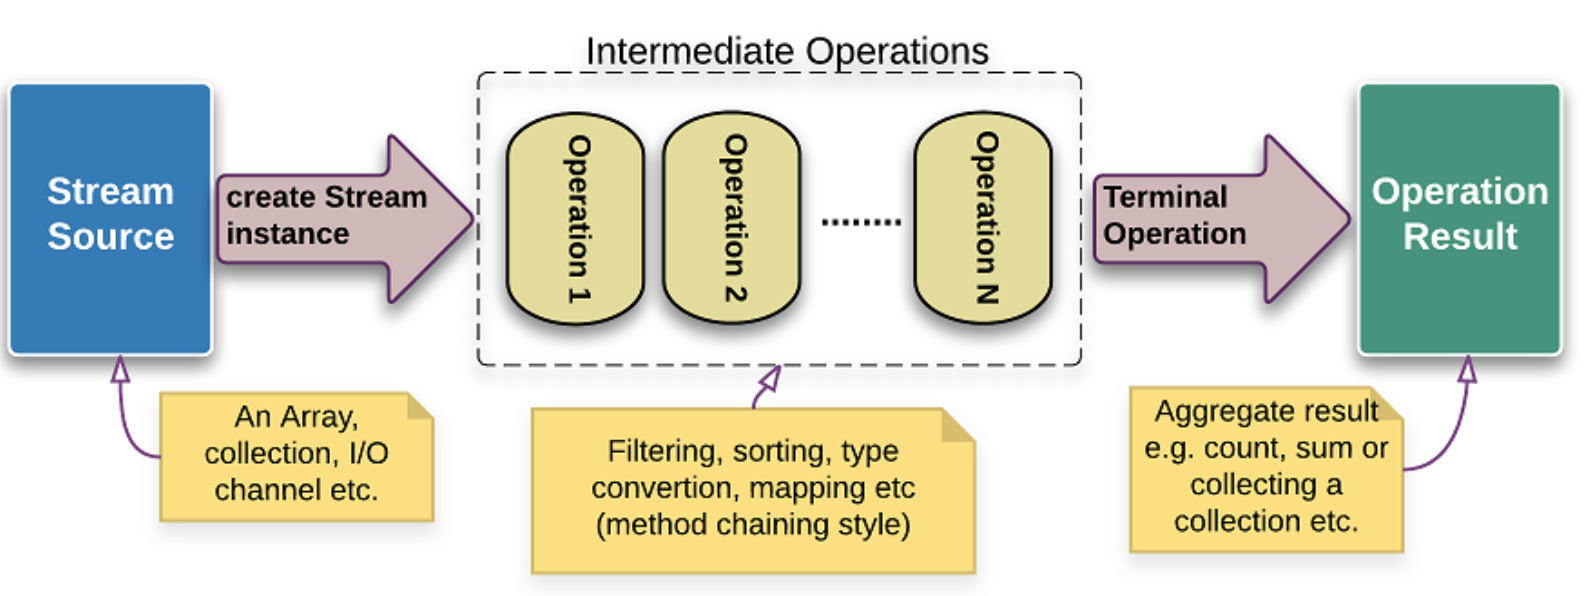
\includegraphics[width=\linewidth]{images/h6/stream_pipeline.png}
  \caption{Stream pipeline (logicbig.com)}
  \label{fig:stream_of}
\end{figure}


De intermediate operators verwerken de elementen van de stream \'e\'en voor \'e\'en. Alle intermediate operations zijn lui (lazy), ze worden enkel uitgevoerd als de stream wordt afgesloten door een terminal operation.

De internal iterator geniet meestal de voorkeur boven de external iterator.  Internal iterations kunnen korter geschreven worden en zijn daardoor ook makkelijker lees- en onderhoudbaar. Toch zijn er situaties, zoals wanneer je 2 verzamelingen gelijktijdig manipuleert, dat je kiest voor een external iterator.

\begin{figure}[H]
  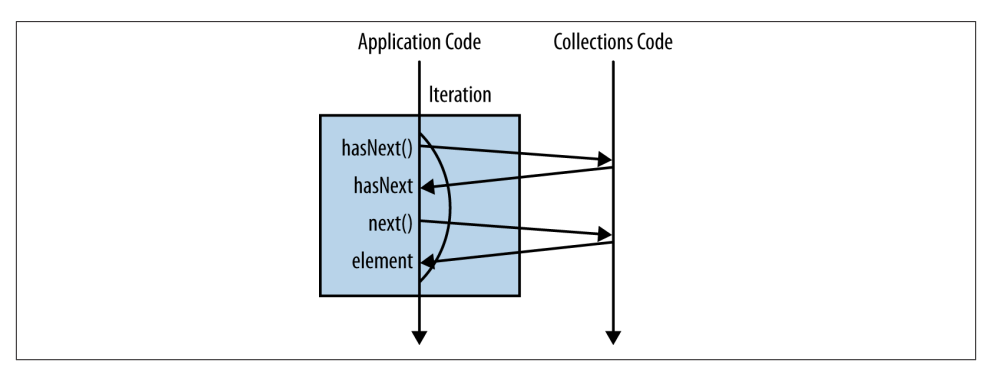
\includegraphics[width=\linewidth]{images/h6/external_iteration.png}
  \caption{External iteration}
  \label{fig:external_iteration}
\end{figure}

\begin{figure}[H]
  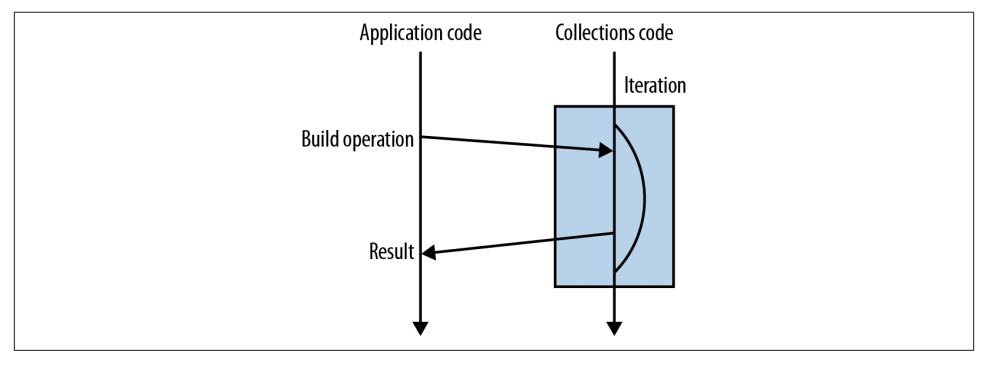
\includegraphics[width=\linewidth]{images/h6/internal_iteration.png}
  \caption{Internal iteration}
  \label{fig:internal_iteration}
\end{figure}



\section{Intermediate en terminal operations}

\subsection{Terminal operation .toList()}

\begin{lstlisting}
import java.util.List;
import java.util.stream.Collectors;
import java.util.stream.Stream;

public class DemoCollect {

	public static void main(String[] args) {

		List<String> theBeatles = 
				Stream.of("John Lennon", "Paul McCartney", "George Harrison", "Ringo Starr")
				.toList();
		System.out.println(theBeatles);
	}

}
\end{lstlisting}

Een stream is geen datastructuur of verzameling. Je moet een stream zien als een reeks objecten. E\'en van de manieren om zo'n reeks of stream te bouwen is met de static methode \textit{of} van de interface Stream.

\begin{figure}[H]
  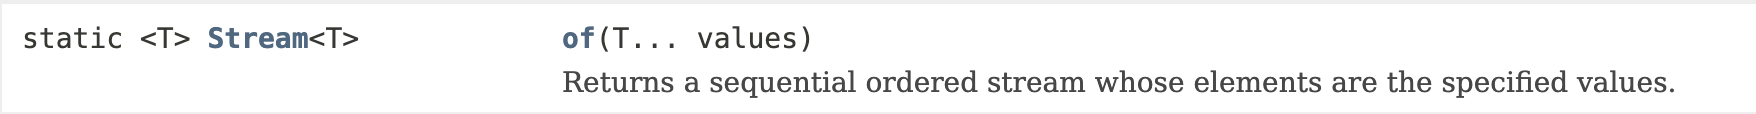
\includegraphics[width=\linewidth]{images/h6/stream_of.png}
  \caption{Static methode of() in de interface Stream}
  \label{fig:stream_of}
\end{figure}

Door gebruik te maken van de operation \textit{.toList()} kunnen we de objecten uit de stream verzamelen in een List.

\subsection{Intermediate operation .filter()}

Wanneer je bepaalde elementen uit een stream wil selecteren, gebruik je een filter. 

\begin{figure}[H]
  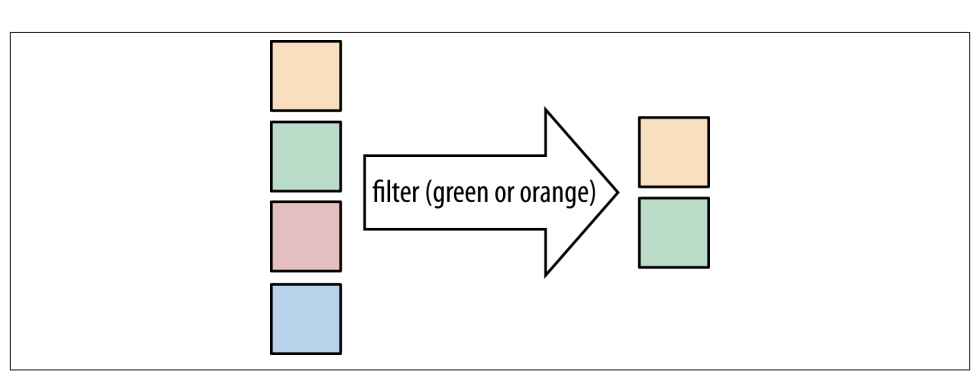
\includegraphics[width=\linewidth]{images/h6/illustration_filter.png}
  \caption{Filter operation}
  \label{fig:filter_operation}
\end{figure}

\begin{figure}[H]
  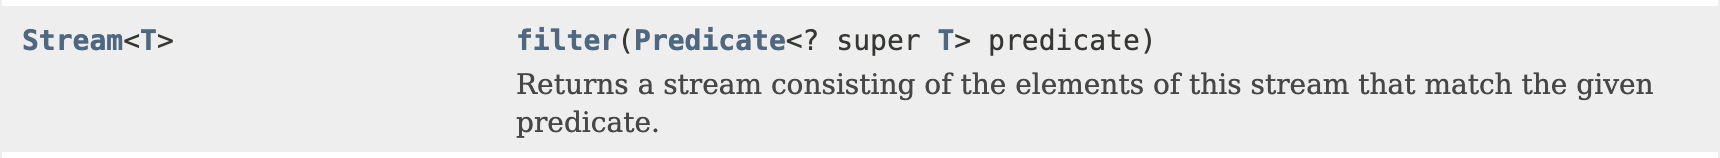
\includegraphics[width=\linewidth]{images/h6/stream_filter.png}
  \caption{Methode filter() in de interface Stream}
  \label{fig:stream_filters}
\end{figure}

Aan de hand van een Predicate wordt beslist welke elementen geselecteerd worden. 

In het onderstaande voorbeeld selecteren we de even getallen uit de verzameling numbers.

\begin{lstlisting}
List<Integer> numbers = Arrays.asList(1,2,3,4,5);

List<Integer> evenNumbers = numbers.stream()
				.filter(n -> n%2  == 0)
				.toList();
				
assertEquals(Arrays.asList(2,4), evenNumbers);
\end{lstlisting}

Nog een voorbeeld:

\begin{lstlisting}
List<String> animals = Stream.of("zebra", "dog", "dolphine")
				.filter(a -> a.contains("o"))
				.toList();

assertEquals(Arrays.asList("dog", "dolphine"), animals);
\end{lstlisting}

Alle String-objecten die een ``o'' bevatten mogen in de stream aanwezig blijven.

Merk op dat de functie filter() een intermediate operation is. De bewerking heeft als return-type Stream. We bouwen als het ware een pipeline. De filter()-operation is ook lazy en zal pas effectief uitgevoerd worden als er een terminal-operation aanwezig is.

Hier volgt nog een voorbeeld met een verzameling met objecten van een zelfgeschreven klasse Participant.

\begin{lstlisting}
public class Participant {
	private String name;
	private int points;

	public Participant(String name, int points) {
		this.name = name;
		this.points = points;
	}

	public int getPoints() {
		return points;
	}

	public String getName() {
		return name;
	}
}
\end{lstlisting}

\begin{lstlisting}
Participant john = new Participant("John P.", 15);
Participant sarah = new Participant("Sarah M.", 200);
Participant charles = new Participant("Charles B.", 150);
Participant mary = new Participant("Mary T.", 1);

List<Participant> participants = Arrays.asList(john, sarah, charles, mary);

List<Participant> over100Points = participants.stream()
     .filter(p -> p.getPoints() > 100)
     .toList();

assertEquals(Arrays.asList(sarah, charles), over100Points);
\end{lstlisting}

Je kan ook meerdere criteria gebruiken in een filter. Je kan in het Predicate de verschillende criteria samenvoegen via boolean operatoren.

\begin{lstlisting}
List<Participant> selection = participants.stream()
    .filter(p -> p.getPoints() > 100 && p.getName().startsWith("S"))
    .toList();
    
assertEquals(Collections.singletonList(sarah), selection);
\end{lstlisting}

Daarnaast kan je ook gebruikmaken van methodes als ``or'',  ``and'' en ``negate'' uit de interface Predicate.
		
\begin{lstlisting}
Predicate<Participant> over100Points = p -> p.getPoints() > 100;
Predicate<Participant> startingWithS = p -> p.getName().startsWith("S");

List<Participant> selection = participants.stream()
    .filter(over100Points.and(startingWithS))
    .toList();

assertEquals(Collections.singletonList(sarah), selection);
\end{lstlisting}

\subsection{Terminal operation .forEach()}

De methode .forEach() is een terminal operation en aanvaardt een implementatie van de functionele interface Consumer als parameter. Deze Consumer beschrijft een actie die met ieder element van de verzameling uitgevoerd zal worden.

\begin{figure}[H]
  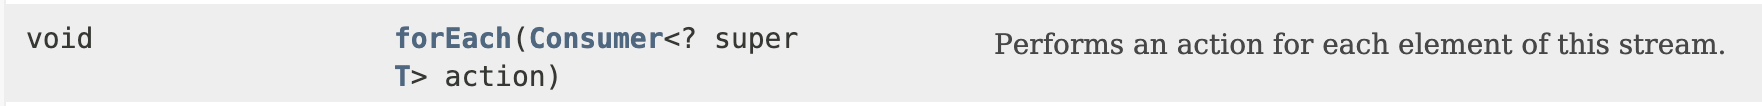
\includegraphics[width=\linewidth]{images/h6/stream_forEach.png}
  \caption{Methode forEach() in de interface Stream}
  \label{fig:stream_foreach}
\end{figure}

\begin{lstlisting}
public class DemoForEach {

	public static void main(String[] args) {
		Participant john = new Participant("John P.", 15);
		Participant sarah = new Participant("Sarah M.", 200);
		Participant charles = new Participant("Charles B.", 150);
		Participant mary = new Participant("Mary T.", 1);

		List<Participant> participants = Arrays.asList(john, sarah, charles, mary);

		participants.stream()
		    .filter(p -> p.getPoints() >= 200)
		    .forEach(System.out::println);

		System.out.println("* All participants *");

		participants.forEach(System.out::println);
	}
}
\end{lstlisting}

Iedere Collection biedt via de interface Iterable ook een forEach methode aan. Met beide forEach functies kan je hetzelfde resultaat bereiken.

\begin{lstlisting}
participants.forEach(System.out::println);
participants.stream().forEach(System.out::println);
\end{lstlisting}

Toch gaat in dit geval onze voorkeur uit naar de eerste optie. Omdat we hier itereren over alle elementen is de stream overbodig.


\subsection{Intermediate operation .map()}

Als je een functie hebt om objecten van \'e\'en datatype te transformeren naar een ander datatype, dan kan je met de bewerking .map(), deze functie loslaten op alle objecten van een stream. 

\begin{figure}[H]
  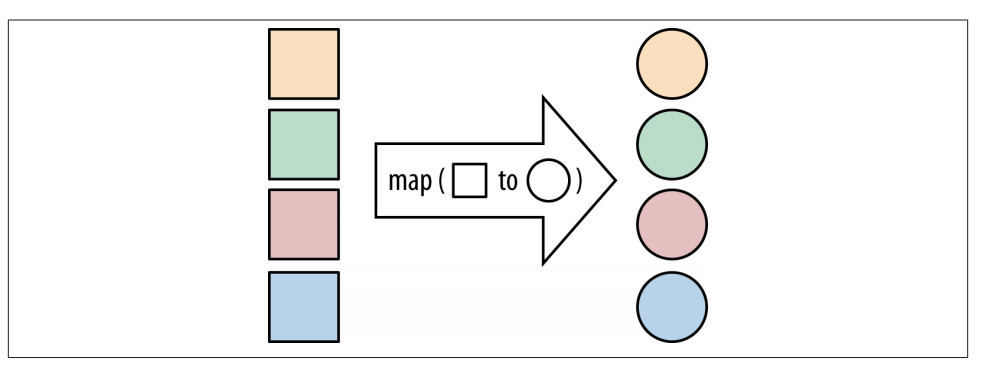
\includegraphics[width=\linewidth]{images/h6/illustration_map.png}
  \caption{Map operation}
  \label{fig:stream_foreach}
\end{figure}

\begin{figure}[H]
  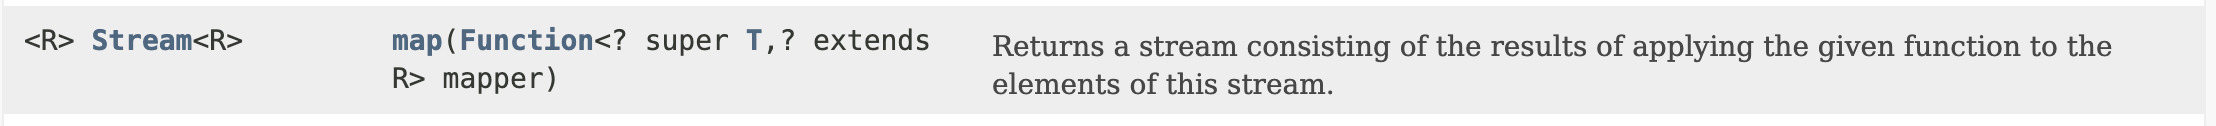
\includegraphics[width=\linewidth]{images/h6/stream_map.png}
  \caption{Methode map() in de interface Stream}
  \label{fig:stream_foreach}
\end{figure}

Map is een lazy operator. Zonder terminal operator zal de meegegeven functie niet uitgevoerd worden, en zal je dus ook geen resultaat krijgen. De functie die je meegeeft aan map is een implementatie van de generieke functionele interface Function$<$T,R$>$.

Hier volgen een twee voorbeelden. In het eerste voorbeeld wijzigt het datatype van de elementen van de stream niet. In het tweede voorbeeld wordt ieder String-object in de stream vervangen door een Integer-waarde.

\begin{lstlisting}
List<String> animals = Stream.of("zebra", "dog", "dolphine")
				.map(String::toUpperCase)
				.toList();

assertEquals(Arrays.asList("ZEBRA", "DOG", "DOLPHINE"), animals);
\end{lstlisting}

\begin{lstlisting}
List<Integer> lengths = Stream.of("zebra", "dog", "dolphine")
				.map(String::length)
				.toList();

assertEquals(Arrays.asList(5, 3, 8), lengths);
\end{lstlisting}

\subsection{Intermediate operation .sorted()}

Wanneer je de intermediate operation sorted() toevoegt aan een stream, worden de elementen in de stream gesorteerd. Zonder parameter zal sorted() de natuurlijke sortering gebruiken. Voor objecten van een zelfgeschreven klasse zorg je er dus voor dat de interface Comparable ge\"implementeerd wordt.

Het is ook mogelijk dat je aan de functie sorted() een parameter meegeeft waarmee je een andere volgorde kan afdwingen. In het tweede voorbeeld gebruiken we niet de natuurlijke (alfabetische) volgorde, maar worden de woorden van lang naar kort gesorteerd.


\begin{lstlisting}
List<String> sortedList = Stream.of("zebra", "dog", "dolphine")
				.sorted()
				.toList();

assertEquals(Arrays.asList("dog", "dolphine", "zebra"), sortedList);
\end{lstlisting}

\begin{lstlisting}
List<String> sortedList = Stream.of("zebra", "dog", "dolphine")
				.sorted((x, y) -> y.length() - x.length())
				.toList();
		
assertEquals(Arrays.asList("dolphine", "zebra", "dog"), sortedList);
\end{lstlisting}

\subsection{Intermediate operation .distinct()}

De operation .distinct() zorgt ervoor dat de elementen in de stream uniek zijn. Elementen die meermaals voorkomen worden verwijderd. Het is de implementatie van de equals() methode (en dus ook hashCode()) van een klasse die beslist of de elementen uniek zijn of niet.

\begin{lstlisting}
List<String> withoutDoubles = Stream.of("zebra", "dog", "zebra", "dolphine")
    .distinct()
    .toList();
    
assertEquals(3, withoutDoubles.size());
\end{lstlisting}

\subsection{Intermediate operation .limit()}

De operation .limit() heeft 1 parameter die het maximaal toegelaten elementen in de stream geeft.
De stream wordt dus als het ware afgekapt.

\begin{lstlisting}
List<String> animals = Stream.of("zebra", "dog", "elephant", "camel", "cat", "fish","dolphine")
    .limit(4)
    .toList();
assertEquals(4, animals.size());
\end{lstlisting}

Met de methode iterate kunnen we een oneindige stream maken. Dankzij de limit(5) worden slechts de eerste 5 nummers gegenereerd.

\begin{lstlisting}
List<Integer> numbers = Stream.iterate(1, n -> n + n)
    .limit(5)
    .toList();

assertEquals(Arrays.asList(1,2,4,8,16), numbers);
\end{lstlisting}


\subsection{Intermediate operation peek()}

De intermediate operation peek kan gebruikt worden om je pipeline te debuggen. Als je wilt controleren welke elementen er op een gegeven moment in de pipeline zitten, dan voeg je peek toe. Zolang je geen terminal operation hebt toegevoegd zal ook peek geen resultaat laten zien.

\begin{lstlisting}
Stream.of("one", "two", "three", "four")
  .filter(e -> e.length() > 3)
  .peek(e -> System.out.println("Filtered value: " + e))
  .map(String::toUpperCase)
  .peek(e -> System.out.println("Mapped value: " + e))
  .toList();
\end{lstlisting}

Je kan de operation peek() verder ook handig gebruiken om de elementen van je stream aan te passen.

\begin{lstlisting}
Stream<User> userStream = Stream.of(new User("Alice"), new User("Bob"), new User("Chuck"));
userStream.peek(u -> u.setName(u.getName().toLowerCase()))
  .forEach(System.out::println);
  \end{lstlisting}


\subsection{Terminal operation .count()}

\begin{lstlisting}
long over100Points = participants.stream().filter(p -> p.getPoints() > 100).count();

assertEquals(2, over100Points);
\end{lstlisting}
		
De terminal operation count gebruik je om het aantal elementen in de stream te tellen.
Indien je geen gebruik maakt van intermediate operations gebruik je de methode size() van je collection om het aantal elementen te achterhalen.

\begin{lstlisting}
System.out.println("Number of participants: " + participants.size());
\end{lstlisting}
		
\section{Intstream, LongStream en DoubleStream}
	
Er zijn ook een aantal afgeleide interfaces van de interface Stream. Deze bieden extra functionaliteit aan. Zo hebben we bijvoorbeeld de interface IntStream, die speciaal ontworpen is voor streams met gehele getallen. Deze stream bevat elementen met datatype \textit{int}. Naast IntStream hebben we ook de interfaces DoubleStream en LongStream. Al deze interfaces bevatten de methoden sum(), min(), max() en average(). 

\subsection{sum()}

Met de operation sum kan je eenvoudig de som berekenen van alle elementen in je stream.

\begin{lstlisting}
long totalPoints = participants.stream().mapToInt(Participant::getPoints).sum();

assertEquals(366, totalPoints);
\end{lstlisting}
		

\subsection{range() en rangeClosed()}
		
De static methoden range() en rangeClosed() zijn beschikbaar in de interfaces java.util.stream.IntStream en java.util.stream.LongStream. Je kan ze gebruiken om een stream te cre\"eren met gehele getallen vanaf een init\"ele waarde tot een stop waarde.
\begin{figure}[H]
  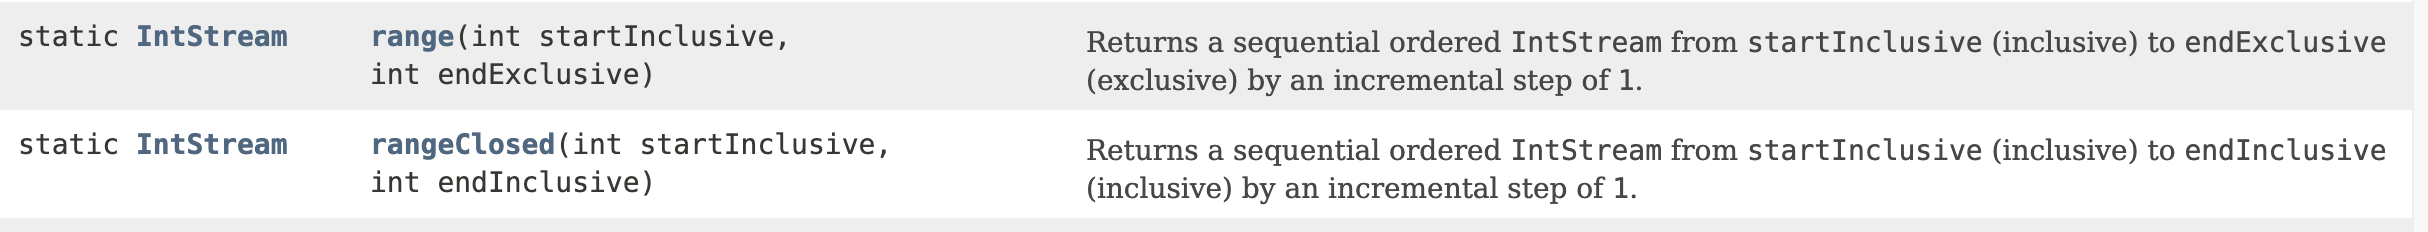
\includegraphics[width=\linewidth]{images/h6/intstream_range.png}
  \caption{Aanmaken van IntStream met range() of rangeClosed()}
  \label{fig:stream_foreach}
\end{figure}

\begin{lstlisting}
long count = IntStream.rangeClosed(10, 20).count();

assertEquals(11, count);
\end{lstlisting}

\subsection{min(), max() en average()}

\begin{figure}[H]
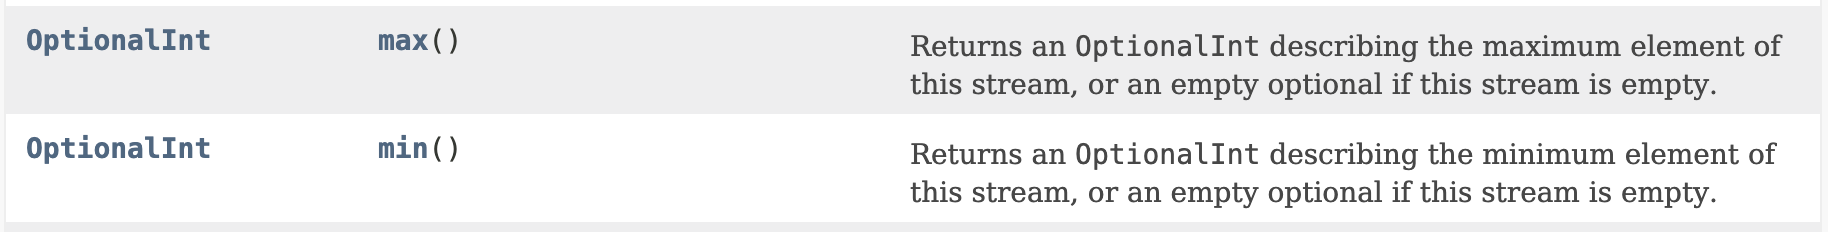
\includegraphics[width=\linewidth]{images/h6/intstream_max_min.png}
\caption{min() en max() uit de interface IntStream}
\label{fig:instream_min_max}
\end{figure}

\begin{figure}[H]
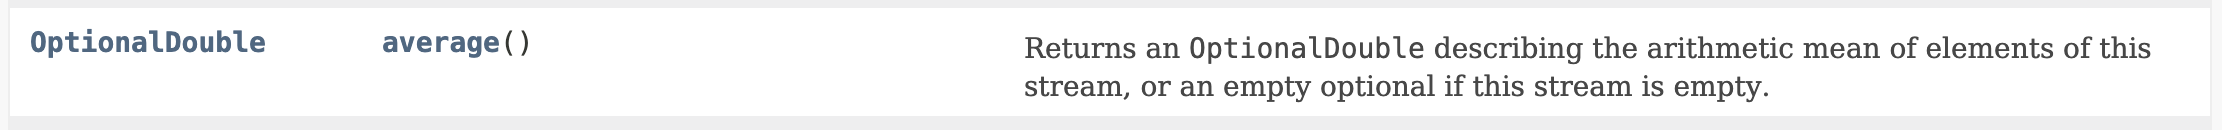
\includegraphics[width=\linewidth]{images/h6/intstream_average.png}
\caption{average() uit de interface IntStream}
\label{fig:instream_average}
\end{figure}

Merk op dat de methoden max() en min() een object van de klasse OptionalInt als return-type hebben. De methode average() heeft OptionalDouble als return-type. 

\begin{oefening}
Zoek de klasse OptionalInt en OptionalDouble op in de Java documentatie.
\end{oefening}

In de documentatie vind je terug dat dit een container-object is dat een int- of double-waarde kan bevatten. Indien we namelijk een lege stream hebben, dan bestaat er immers geen minimum, maximum of gemiddelde. In plaats van bijvoorbeeld een exception op te gooien wanneer we max() oproepen voor een lege IntStream, is er gekozen om steeds een OptionalInt als resultaat te geven. Bij een lege IntStream bevat het OptionalIInt-object geen waarde en \textit{isPresent()} geeft false als resultaat. Indien er wel een maximum berekend kan worden geeft \textit{isPresent()} true. De berekende waarde kan je bekomen via de methode \textit{getAsInt()}.

\begin{lstlisting}
Random random = new Random();
List<Integer> randomNumbers = random.ints(15, 0, 100).boxed().toList();
int max = randomNumbers.stream().mapToInt(x -> x).max().getAsInt();
int min = randomNumbers.stream().mapToInt(x -> x).min().getAsInt();
double average = randomNumbers.stream().mapToInt(x -> x).average().getAsDouble();
assertTrue(min <= average);
assertTrue(max >= average);

IntSummaryStatistics intSummaryStatistics = random.ints(15, 0, 100).summaryStatistics();
assertTrue(intSummaryStatistics.getMax() >= intSummaryStatistics.getMin());
\end{lstlisting}


\section{Method reference}

Method references zijn een speciaal type lambda expressies. Ze worden gebruikt om lambda expressies te vereenvoudigen door te verwijzen naar een bestaande methode, zonder dat je expliciet de parameters moet invullen.

Er zijn 4 soorten methodes in Java:
\begin{itemize}
\item static methods
\item constructoren
\item instance methods
\end{itemize}

\subsection{Static methods}
Syntax: 
\begin{verbatim}
ClassName::staticMethod
\end{verbatim}

\begin{lstlisting}
IntBinaryOperator min = (x, y) -> Math.min(x, y);
IntBinaryOperator max = Math::max;

System.out.println(min.applyAsInt(-3, 17));
System.out.println(max.applyAsInt(-3, 17));
\end{lstlisting}



\subsection{Instance method (unbounded)}
Syntax:
\begin{verbatim}
ClassName::instanceMethod
\end{verbatim}

\begin{lstlisting}
Function<String, String> toUpperCase = s -> s.toUpperCase();
Function<String, String> toLowerCase = String::toLowerCase;
System.out.println(toUpperCase.apply("abcdef"));
System.out.println(toLowerCase.apply("ABCDEF"));
\end{lstlisting}

\subsection{Instance method (bounded)}

Syntax:
\begin{verbatim}
instance::instanceMethod
\end{verbatim}

De klasse Random voorziet 2 versies van de methode nextInt(): een eerste versie zonder parameter en een tweede versie met \'e\'en parameter, de bovengrens. Dit principe noemen we methode overloading. Aan de hand van de functionele interface die je implementeert, kan je nu de gewenste methode als en lambda functie schrijven. Hier illustreren we hoe je deze lambda functie ook nog eens verkort kan schrijven door gebruik te maken van method reference.

\begin{lstlisting}
Random random = new Random();
IntSupplier randomInt = random::nextInt;
IntUnaryOperator randomIntWithBound = random::nextInt;
System.out.println(randomInt.getAsInt());
System.out.println(randomIntWithBound.applyAsInt(12));
\end{lstlisting}

\subsection{Constructor}

Je kan ook voor een constructor een method reference maken. De syntax van de method reference voor een constructor ziet er als volgt uit.

\begin{verbatim}
ClassName::new
\end{verbatim}

\begin{lstlisting}
System.out.println("Constructor");
Supplier<Random> randomCreator = Random::new;
Random random = randomCreator.get();
\end{lstlisting}

\begin{lstlisting}
public class Person {
    private String name;

    public Person() {
        this.name = "Unknown";
    }

    public Person(String name) {
        this.name = name;
    }

    public String getName() {
        return name;
    }
}
\end{lstlisting}

\begin{lstlisting}
public class ConstructorMethodReferenceExample {
    public static void main(String[] args) {
        // Using a constructor method reference to create a new Person object
        Supplier<Person> personSupplier = Person::new;
        Person person = personSupplier.get();
        System.out.println("Name: " + person.getName()); // Outputs: Name: Unknown
   
        // Using a constructor method reference to create a new Person object with a name
        Function<String, Person> personFunction = Person::new;
        Person person2 = personFunction.apply("Alice");

        System.out.println("Name: " + person2.getName()); // Outputs: Name: Alice
    }
}
\end{lstlisting}

\begin{oefening}

In de klasse be.pxl.ja.oefening1.StudentList vind je een static methode createStudents(). Voorzie nu een hoofdprogramma waarin je start met deze lijst en de volgende vragen beantwoordt met behulp van een stream.

\begin{itemize}
\item Welke studenten zijn er vandaag jarig. Toon hun naam. Je verandert best een geboortedata van de studenten om je stream uit te testen.
\item Toon alle gegevens van de student met de naam Carol.
\item Hoeveel studenten studeerden af in 2017?
\item Wat is de hoogste score ooit behaald? Wie behaalde deze hoogste score ooit?
\item Wie is de oudste persoon in de lijst?
\item Geef de namen van alle studenten gescheiden door komma (,) in  \'e\'en String.
\item Wie is de jongste student van afstudeerjaar 2018?
\item Maak een map met per afstudeerjaar de gemiddelde score.
\item Sorteer de studenten eerst op afstudeerjaar (recentste jaar eerst) en per afstudeerjaar volgens hun score (van hoog naar laag). Toon naam, afstudeerjaar en score.
\end{itemize}
\end{oefening}
